\documentclass[
	classe=$2^{de}$
]{exercice}

\usepackage{tikz-repère}
\usepackage{tkz-tab}

\title{Activité : trois fonctions}

\begin{document}

\maketitle

On a tracé dans le repère ci-dessous le graphe de trois fonctions $f$, $g$ et $h$ :

\newcommand{\functionF}[1]{
	(1/27)*#1*#1*#1 - #1
}
\newcommand{\functionG}[1]{
	(#1 - 4.24) / ((#1-0.24)*(#1-0.24) + 2) + 4.06
}
\newcommand{\functionH}[1]{
	-#1*#1/3 + 6.33
}
\begin{center}
	\begin{tikzpicture}
		\tikzRepere{-5.5}{5.5}{-2.5}{6.5}

		\newcommand{\DessineFonction}[5]{
			\pgfmathsetmacro\TEMP{#4-1}
			\foreach \n in {#3,...,\TEMP} {
					\draw[domain=\n:\n+1,very thick,#5] plot({\x},{#2});
				}
			\draw[domain=#4-1:#4,very thick,#5] plot({\x},{#2}) node[right] {#1};
		}
		\DessineFonction{$f$}{\functionF{\x}}{-6}{6}{blue}
		\DessineFonction{}{(\x+4.8)*(\x+4.8)/5.67 + 3.74}{-6}{-5}{red}
		\DessineFonction{$g$}{\functionG{\x}}{-5}{3.5}{red}
		\DessineFonction{}{\functionH{\x}}{-5}{-1}{green}
		\DessineFonction{$h$}{\functionH{\x}}{1}{5}{green}
	\end{tikzpicture}
\end{center}

\begin{enumerate}
	\item Lire les valeurs de $f(3)$, $g(0)$ et $h(4)$.

	      \correction{$-2$, $2$ et $1$}
	\item Quel est le domaine de définition de chacune de ces fonctions ?

	      \correction{$\intervalle{[}{-6}{6}{]}$, $\intervalle{[}{-6}{3,5}{]}$ et $\intervalle{[}{-5}{-1}{]}∪\intervalle{[}{1}{5}{]}$}
	\item Remplir les tableaux de variations suivants :

	      \begin{center}
		      \begin{tikzpicture}[scale=0.8]
			      \tkzTabInit{$x$ / 1 , $f(x)$ / 2}{$\correction{-6}$, $\correction{-3}$, $\correction{3}$, $\correction{6}$}
			      \ifdefined\makeCorrection
				      \tkzTabVar{-/ $-2$, +/ $2$, -/ $-2$, +/ $2$}
			      \fi
		      \end{tikzpicture} \medskip

		      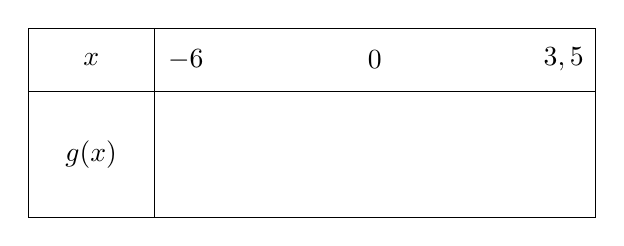
\begin{tikzpicture}[scale=0.8]
			      \tkzTabInit{$x$ / 1 , $g(x)$ / 2}{$\correction{-6}$, $\correction{0}$, $\correction{3,5}$}
			      \ifdefined\makeCorrection
				      \tkzTabVar{+/ $4$, -/ $2$, +/ $4$}
			      \fi
		      \end{tikzpicture} \medskip

		      \begin{tikzpicture}[scale=0.8]
			      \tkzTabInit{$x$ / 1 , $h(x)$ / 2}{$\correction{-5}$, $\correction{-1}$, $\correction{1}$, $\correction{5}$}
			      \ifdefined\makeCorrection
				      \tkzTabVar{-/ $-2$, +H/ $6$, +/ $6$, -/ $-2$}
			      \fi
		      \end{tikzpicture}
	      \end{center}
\end{enumerate}

\end{document}